\part{Vision}


\section{Conics and quadrics}

\subsection{Ellipses}
The general quadratic equation of a conic is: $Ax^2 + Bxy + Cy^2 + Dx + Ey + F = 0 $

It can be written in the homogeneous form:
\begin{equation}
(x~~y~~1) \left[\begin{array}{ccc}
     A & B/2 & D/2  \\
     B/2 & C & E/2 \\
     D/2 & E/2 & F
\end{array}\right] 
\left( \begin{array}{c}
     x  \\
     y \\
     1
\end{array} \right)
= 0
\end{equation}
In 2D projective geometry, all conics are equivalent under a projective transformation.

An ellipse is a specific form of conic and has the equation:
\begin{equation}
\frac{x^2}{a^2} + \frac{y^2}{b^2} = 1
\end{equation}

\subsubsection{Euclidean matrix form}
\begin{equation}
    (X - C)^T A (X - C) = 1
\end{equation}
$C$ is the ellipse center and $A$ is a 2x2 symmetric matrix defining its shape. The eigen vectors of $A$ are the two axes and their corresponding eigen values give $1/a^2$ and $1/b^2$.

It is possible to extract the rotation part out of $A$:
\begin{equation}
(X - C)^T {}^{e}R_{w}^T \left[ \begin{array}{cc}
    1/a^2 & 0 \\
    0 & 1/b^2
\end{array}
\right] {}^{e}R_{w} (X - C) = 1
\end{equation}

\subsubsection{Homogeneous form}
\begin{equation}
    X^T T_{-C}^T
    {}^{e}R_{w}^T
    \left[ \begin{array}{ccc}
    1/a^2 & 0 & 0\\
    0 & 1/b^2 & 0\\
    0 & 0 & -1
    \end{array}\right]
    {}^{e}R_{w}
    T_{-C}
    X = 0
\end{equation}

where $T_{-C} = \left[\begin{array}{ccc}
    1&0&-C_x \\
    0&1&-C_y \\
    0&0&1
    \end{array}\right]$ is a translation to move the ellipse center to~(0, 0).

This gives a complete homogeneous equation:
\begin{equation}
    X^T C X = 0
\end{equation}
where $C$ is a 3x3 symmetric matrix defined up to a scale (6 elements for only 5 parameters because of the scale).

\subsubsection{Dual form}
It defines the ellipse by tangent lines instead of points. It satisfies:
\begin{equation}
    l^T C^* l = 0
\end{equation}

where $C^*$ is the adjointe matrix (conjugate transpose) of $C$ and we have $C^* \sim C^{-1}$

\subsubsection{Decompose an ellipse}
This show how to decompose an ellipse into: half-axes, orientation and center.
\begin{algorithm}[H]
\DontPrintSemicolon
\KwInput{$C$: dual-form 3x3 matrix of the ellipse}
\KwOutput{half-axes, orientation, center}
 $C/-C[2, 2]$ \tcp*{normalize by minus C[2, 2] (force C[2, 2] = -1)}
 $c = -C[:2, 2]$  \tcp*{is the center of the ellipse}
 $C_{centered} = T_{-c} C T_{-c}^T $ \tcp*{Get the ellipsoid centered}
 $C_{centered} = 0.5\times(C_{centered}+C_{centered}^T)$ \tcp*{Enforce symmetry}
 $D, R = eig(C_{centered}[:2, :2])$ \tcp*{Eigen decomposition}
 $a, b = sqrt(abs(D))$, $orientation = R$, $center = c$
\caption{Decompose ellipse}
\end{algorithm}


\subsubsection{Fitting an ellipse}
see \href{https://members.loria.fr/MOBerger/Enseignement/Master2/Documents/ZhangIVC-97-01.pdf}{Zhang}

\paragraph{Least-squares fitting based on algebraic distance}

This is the easiest way to fit an ellipse because it has closed-form solution. With ideal points, we would like to have the \textit{algebraic distance} equal to 0: $Q(x_i, y_i) =  Ax_i^2 + Bx_iy_i + Cy_i^2 + Dx_i + Ey_i + F = 0$.
Because of noise, this equation is not true, so we want to minimize the following \textit{objective function}.

\begin{equation}
    F = \sum_{i=1}^{n} Q^2(x_i, y_i)
\end{equation}

Clearly, there is a trivial solution: $A=B=C=D=E=F=0$. Let $p = [A, B, C, D, E, F]^T$. To avoid the trivial solution, we need to normalize $p$. Different normalization are possible: $\norm{p} = 1$, $A + C = 1$, $F = 1$.

\paragraph{Normalization: $\norm{p}=1$}

An ellipse have 5 degrees of freedom (3x3 symmetric matrix: 6 parameters -1 for the scale).

Each point gives one equation, so we need at least 5 points.
\begin{equation}
    \left[
    \begin{array}{cccccc}
    x_i^2 & x_i y_i & y_i^2 & x_i & y_i & 1  \\
    \vdots &\vdots &\vdots &\vdots &\vdots &\vdots 
    \end{array}
    \right]
    \left[\begin{array}{c}
        a \\ b \\ c \\ d \\ e \\ f
    \end{array} \right]
    = 0
\end{equation}

solve this homogeneous system $Ax=0$ with SVD. The last row of $Vt$ gives the best estimation.

\paragraph{Normalization: $A + C = 1$}
The trace of the conic matrix $A + C$ can never be 0, so we can force $A + C = 1$.
With this normalization, all ellipses can be expressed by 5 parameters: $p = [A, B, D, E, F]^T$. So, we minimize $\norm{Ap-b}$,

\begin{equation}
    \left[
    \begin{array}{ccccc}
    x_i^2 - y_i^2 & x_i y_i & x_i & y_i & 1  \\
    \vdots &\vdots &\vdots &\vdots &\vdots 
    \end{array}
    \right]
    \left[\begin{array}{c}
        a \\ b \\ d \\ e \\ f
    \end{array} \right]
     - 
    \left[\begin{array}{c}
        -y_i \\
        \vdots
    \end{array} \right]
\end{equation}


The solution to $Ap=b$ is given by the \textit{pseudo-inverse}: $p = (A^T A)^{-1} A^T b$


\paragraph{Normalization: $F = 1$}
This is another used normalization. However, this normalization has singularities for all conics going through the origin because $F = 0$.


\paragraph{Least-squares fitting based on Euclidean distance}

The methods based on algebraic distance have the advantage of begin simple and having closed-form solution. However, they introduce a bias where points on regions of high curvature have less impact than points on regions of low curvature.

Methods based on Euclidean distance are better but are based on the minimization of an orthogonal distance to the ellipse which is complicated to compute and requires iterative methods for minimization.



\subsection{Ellipsoids}

Ellipsoids are quadrics with the following type of equation:
\begin{equation}
    \frac{x^2}{a^2} + \frac{y^2}{b^2} + \frac{z^2}{c^2} = 1
\end{equation}


\subsubsection{Euclidean matrix form}
Similar to the ellipse case, the general Euclidean form of an ellipsoid is:
\begin{equation}
    (X - C)^T A (X - C) = 1
\end{equation}
$C$ is the ellipse center and $A$ is a 3x3 symmetric matrix defining its shape. The eigen vectors of $A$ are the three axes and their corresponding eigen values give $1/a^2$, $1/b^2$ and $1/c^2$.

Again, it is possible to extract the rotation out of $A$:

\begin{equation}
(X - C)^T {}^{e}R_{w}^T \left[ \begin{array}{ccc}
    1/a^2 & 0 & 0 \\
    0 & 1/b^2 & 0 \\
    0 & 0 & 1/c^2
\end{array}
\right] {}^{e}R_{w} (X - C) = 1
\end{equation}


\subsubsection{Homogeneous form}
\begin{equation}
    X^T T_{-C}^T
    {}^{e}R_{w}^T
    \left[ \begin{array}{cccc}
    1/a^2 & 0 & 0 & 0\\
    0 & 1/b^2 & 0 & 0\\
    0 & 0 & 1/c^2 & 0\\
    0 & 0 & 0 & -1
    \end{array}\right]
    {}^{e}R_{w}
    T_{-C}
    X = 0
\end{equation}

where $T_{-C} = \left[\begin{array}{cccc}
    1&0&0&-C_x \\
    0&1&0&-C_y \\
    0&0&1&-C_z \\
    0&0&0&-1
    \end{array}\right]$ is a translation to move the ellipsoid center to~(0, 0, 0).

This gives a complete homogeneous equation:
\begin{equation}
    X^T Q X = 0
\end{equation}

where $Q$ is a 4x4 symmetric matrix defined up to a scale (10 elements for only 9 parameters because of the scale).

\subsubsection{Dual form}
It defines the ellipsoid by tangent planes instead of points. It satisfies:
\begin{equation}
    l^T Q^* l = 0
\end{equation}

where $Q^*$ is the adjointe matrix (conjugate transpose) of $Q$ and we have $Q^* \sim Q^{-1}$


\subsubsection{Decompose an ellipsoid}
This show how to decompose an ellipsoid into: half-axes, orientation and center.

\begin{algorithm}[H]
\DontPrintSemicolon
\KwInput{$Q$: dual-form 4x4 matrix of the ellipsoid}
\KwOutput{half-axes, orientation, center}
 $Q/-Q[3, 3]$ \tcp*{normalize by minus Q[3, 3] (force Q[3, 3] = -1)}
 $c = -Q[:3, 3]$  \tcp*{is the center of the ellipsoid}
 $Q_{centered} = T_{-c} Q T_{-c}^T $ \tcp*{Get the ellipsoid centered}
 $Q_{centered} = 0.5\times(Q_{centered}+Q_{centered}^T)$ \tcp*{Enforce symmetry}
 $D, R = eig(Q_{centered}[:3, :3])$ \tcp*{Eigen decomposition}
 $a, b, c = sqrt(abs(D))$, $orientation = R$, $center = c$
\caption{Decompose ellipsoid}
\end{algorithm}

\section{2D Transformations}

\begin{tabular}{|c|c|c|c|}
 \hline
  Transformation & degrees of freedom & matrix & invariants \\
  \hline
  Projective & 8 dof & 
  $\left[\begin{array}{ccc}
       h_{11}&h_{12}&h_{13}  \\
       h_{21}&h_{22}&h_{23}  \\
       h_{31}&h_{32}&h_{33}  \\
    \end{array}\right]$ & 
    \begin{minipage}[t]{0.4\textwidth}
    \begin{itemize}
        \item lines (collinearity)  
        \item cross ratios (ratio of ratio)
    \end{itemize}
    \end{minipage}
    \\
    \hline
    
      Affine & 6 dof & 
  $\left[\begin{array}{ccc}
       a_{11}&a_{12}&t_{x}  \\
       a_{21}&a_{22}&t_{y}  \\
       0 & 0 & 1  \\
    \end{array}\right]$ & 
    \begin{minipage}[t]{0.4\textwidth}
    \begin{itemize}
        \item parallelism
        \item centroid
        \item line/point at infinity
    \end{itemize}
    \end{minipage}
    \\
    \hline
    
    Similarity & 4 dof & 
  $\left[\begin{array}{ccc}
       sr_{11}&sr_{12}&t_{x}  \\
       sr_{21}&sr_{22}&t_{y}  \\
       0 & 0 & 1  \\
    \end{array}\right]$ & 
    \begin{minipage}[t]{0.4\textwidth}
    \begin{itemize}
        \item angles
        \item ratio of length
        \item ratio of areas
    \end{itemize}
    \end{minipage}
    \\
    \hline
    
       Isometry (Euclidean) & 3 dof & 
  $\left[\begin{array}{ccc}
       r_{11}&r_{12}&t_{x}  \\
       r_{21}&r_{22}&t_{y}  \\
       0 & 0 & 1  \\
    \end{array}\right]$ & 
    \begin{minipage}[t]{0.4\textwidth}
    \begin{itemize}
        \item length
        \item angles
    \end{itemize}
    \end{minipage}
    \\
    \hline
\end{tabular}

\textbf{\underline{Note:}}

A similarity transform can be decomposed as a rotation $\theta$ and a non-uniform scaling $D$ with a certain orientation $\phi$:  $S = R(\theta)R(-\phi)DR(\phi)$

The group of invertible nxn matrices is the \textit{General Linear Group}.

The projective transform is the only kind of transform that can move points/lines at infinity to finite points/lines or vice versa.

The \textit{Projective Linear Group} is a subgroup of the matrices which are equivalent by a scalar factor.


\subsection{Topology of the projective plane}
Any point can be normalized such that: $x_1^2 + x_2^2 + x_3^2 = 1$.
Such point lies on the unit sphere $S^2$ in $R^3$
There is a 2-to-1 correspondence between $S^2$ and $P^2$.
Opposite points on the sphere represent the same point. Any two points on the sphere lies on a single great circle which correspond to the line between the two points. Any two great circles intersect into a single points (in fact 2 opposite points which represent the same point).

\subsubsection{Homogenous representation of points}
The homogeneous representation of a point is :
\begin{equation}
    \textbf{p} \sim \left(\begin{array}{c}
        \bar{p}\\1
    \end{array}\right)
    =
    \left(\begin{array}{c}
        x\\y\\1
    \end{array}\right)
\end{equation}

\textbf{P-normalization}
The mapping $R^2 \rightarrow P^2$ has an inverse mapping obtained by normalization.
\begin{equation}
    \textbf{x} = \left(\begin{array}{c}
        x_1 \\ x_2 \\ x_3
    \end{array}\right)
\end{equation}
and
\begin{equation}
    \textbf{x} \sim \left(\begin{array}{c}
        x_1 / x_3 \\ x_2 / x_3 \\ 1
    \end{array}\right)
\end{equation}


\subsubsection{Homogenous representation of lines}
Equation of a line in 2D: $l_1x + l_2y - \Delta = 0$

In homogeneous coordinates the line becomes:
\begin{equation}
    \textbf{l} \sim \left(\begin{array}{c}
        l_1 \\ l_2 \\ -\Delta
    \end{array}\right)
\end{equation}
In the canonical form, we assume $l_1^2 + l_2^2 = 1$ and $\Delta \ge 0$.
The previous equation becomes: $x^Tl=0$.


\textbf{D-normalization}
\begin{equation}
    \textbf{l} = \left(\begin{array}{c}
        \beta_1 \\ \beta_2 \\ \beta_3
    \end{array}\right)
\end{equation}

To go back to the canonical form, we do:
\begin{equation}
    \textbf{l}\sim \frac{-sign(\beta_3)}{\sqrt{\beta_1^2+\beta_2^2}} \left(\begin{array}{c}
        \beta_1 \\ \beta_2 \\ \beta_3
    \end{array}\right)
    = \left(\begin{array}{c}
        l_1 \\ l_2 \\ -\Delta
    \end{array}\right)
\end{equation}



\section{Gaussian and $\chi^2$ distributions}
\subsubsection{Gaussian probability distribution}
Given a vector $X$ of random variables $x_i$ for $i=1,\dots,N$, with mean $\bar{X} = E[X]$, and $\Delta_X = X - \bar{X}$, the covariance matrix $\Sigma$ is a NxN matrix given by

\begin{equation}
    \Sigma = E[\Delta_X \Delta_X^T]
\end{equation}

so that $\Sigma_{ij}=E[\Delta_{x_i}\Delta_{y_i}]$. The diagonal elements of $\Sigma$ are the variances of the individual variables $x_i$, and the off-diagonal elements are the cross-variances values.
In non-degenerate cases, where $\Sigma$ is positive-definite and thus invertible, the multivariate Gaussian distribution is
\begin{equation}
P(X)=\frac{1}{(2\pi)^{N/2}|\Sigma|^{1/2}} e^{-\frac{1}{2}(X-\bar{X})^T \Sigma^{-1} (X-\bar{X})}
\end{equation}

where $|\Sigma|$ is the determinant of $\Sigma$.

In the case where $\Sigma$ is just a diagonal matrix with a unique scalar term on the diagonal, $\Sigma=\sigma^2 I$, the distribution is called an \textit{isotropic Gaussian distribution}.

\subsubsection{Mahalanobis distance}

It is defined as:
\begin{equation}
    \norm{X - Y}_{Sigma}=\sqrt{(X-Y)^T \Sigma^{-1} (X-Y)}
\end{equation}{}

where $\Sigma$ is a positive definite matrix. This defines a metrix on $R^N$.
We can see that the Gaussian distribution is equivalent (without the normalization terms) to 

\begin{equation}
    P(X) \approx e^{-\frac{\norm{X-\bar{X}}_{\Sigma}^{2}}{2}}
\end{equation}{}

\subsubsection{Change of coordinates}
Since $\Sigma$ is symmetric and positive-definite, it may be rewritten as $\Sigma=U^T D U$, where $U$ is an orthogonal matrix and $D=(\sigma_1^2, \sigma_2^2, \dots, \sigma_N^2)$ is diagonal.

This shows that a general Gaussian PDF can be changed into an \textit{isotropic Gaussian distribution} with an orthogonal change of coordinates $X^\prime = UX$ and a scaling $\sigma_i$ of each component.
This also show that Euclidean distance and Mahalanobis distances are equivalent under a change of coordinates.

\subsection{$\chi^2$ distribution}

The $\chi_n^2$ distribution is the distribution of the sum of squares of $n$ independant Gaussian random variables. For a Gaussian random vector $v$, the value ${(v-\bar{v})^T \Sigma^{-1} (v-\bar{v})}$ satisfies a $\chi_n^2$ distribution, where $n$ is the dimension of $v$.



\section{Algorithm evaluation and error analysis}
\underline{Convention}
$x$ represents a measured image point.
Estimated quantities are represented with a hat, $\hat{x}$ or $\hat{H}$.
True values are represented with a bar, $\bar{x}$ or $\bar{H}$.

In the following subsections, we treat the problem of estimating a projective transformation between 2D points.

\subsection{Error in one image}

Suppose the points in the first image are noise-free $x_i = \bar{x}_i$ and points in the second image $x^\prime_i$ have a Gaussian noise. After estimating the transform $\hat{H}$, we can compute a \textit{residual error} which gives the average difference between the noisy input data $x^\prime_i$ and the 
estimated points $\hat{x}^\prime_i = \hat{H}\bar{x}_i$

\begin{equation}
    \epsilon_{res} = \sqrt{\left( \frac{1}{2n}\sum_{i=1}^{n} d(x^\prime_i,\hat{x}^\prime_i)^2 \right)}
\end{equation}{}

In case of only 4 points, the estimated homography will perfectly fit the noisy input data and thus the residual error will be 0. However, this estimation will not be very close approximation to the noise-free values.
With more than 4 points, the residual error will increase, but the estimated model will agree more and more with the noise-free true values.

\subsection{Error in both images}
In case of errors in both images, the residual error becomes

\begin{equation}
    \epsilon_{res} = \frac{1}{\sqrt{4n}} \sqrt{\sum_{i=1}^{n} d(x_i, \hat{x}_i)^2 + \sum_{i=1}^{n} d(x^\prime_i, \hat{x}^\prime_i)^2}
\end{equation}{}

where $\hat{x}_i$ and $\hat{x}_i^\prime$ are estimated points such that $\hat{x}_i = \hat{H} \hat{x}_i^\prime$.


\subsection{Optimal estimators (MLE)}
Maximum Likelihood Estimator (MLE) gives a theoretical optimal solution and any other algorithm should be compared to it.
A general estimation problem is with function $f$ from $R^M$ to $R^N$ where $R^M$ is a parameter space and $R^N$ is a space of measurements. Consider a point $\bar{X}$ from the measurement space for which there exists a point $\bar{P}$ in the parameters space such that $f(\bar{P}) = \bar{X}$. In case of homography between 2 sets of $n$ points, $\bar{X}$ contains its $N=2n$ coordinates and $\bar{P}$ contains the 8 or 9 parameters of the homography.

Let $X$ be a measurement chosen according to an isotropic Gaussian distribution of mean $\bar{X}$ and total variance $N\sigma^2$ (this is the sum of the variance of each component = trace of the covariance matrix).

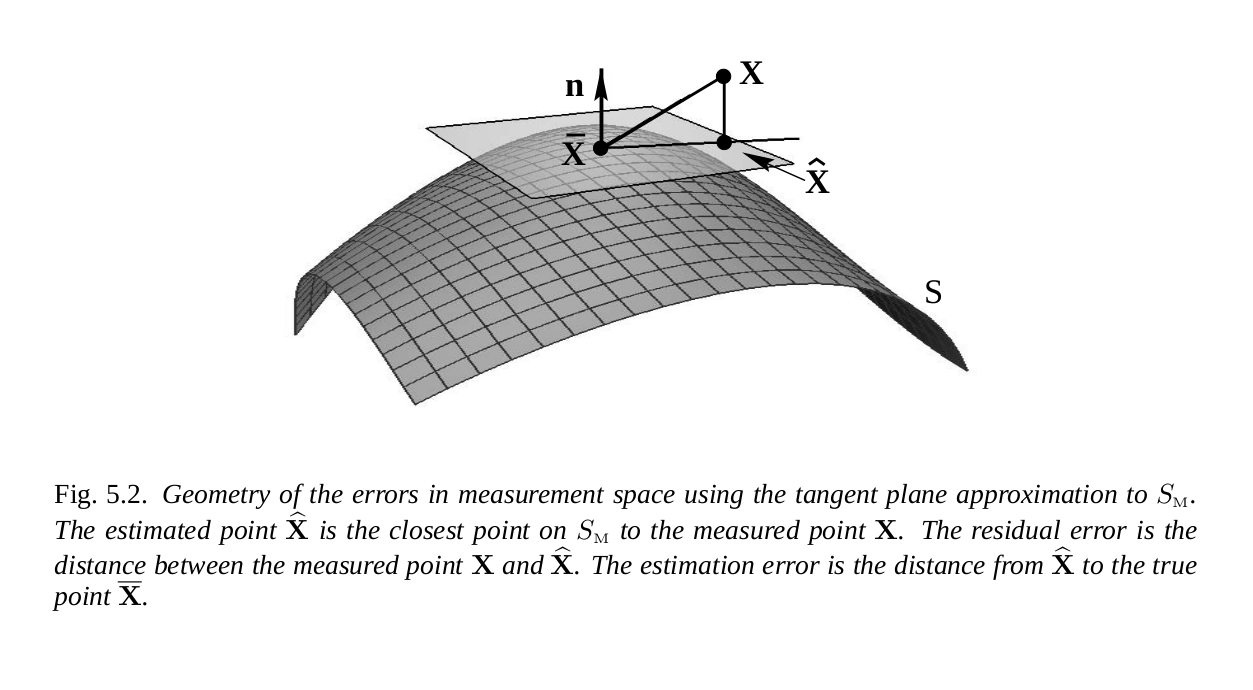
\includegraphics[scale=0.25]{content/MLE.png}

As the value of the parameter vector $P$ varies in a neighbourhood of $\bar{P}$, the values of $f(P)$ traces out a surface $S_m$ in $R^N$ through point $\bar{X}$. This surface is a sub-manifold of $R^N$ and has dimension $d$, the number of essential parameters (= nb of degrees of freedom or minimum number of parameters). The ML estimate $\hat{X}$ is the point on the curve which is the closest to the measurement point $X$.

If we assume that in a neighbourhood of $\bar{X}$, the surface is planar, this ML estimate is the orthogonal projection of $X$ onto the plane.
The residual error corresponds to the distance between $X$ and $\hat{X}$. Its distribution is the projection of the distribution of the Gaussian distribution variable on the $N-d$-dimensional normal of the plane.
The estimator error corresponds to the distance between $\bar{X}$ and $\hat{X}$. Its distribution is projection of the distribution of the Gaussian random variable onto the $d$-dimensional plane.

With this its possible to compute the \textbf{expected residual errors} and the \textbf{expected estimator error}.

\subsection{Covariance of estimation}

We saw in the previous subsection that the achievable residual error and estimation error depends only on the number of points correspondence and their accuracy. However, the confidence of the estimation (its covariance) depends also on the configuration off the points. For example, if we take 4 points almost collinear, the behaviour of the transformation along the perpendicular dimension cannot be accurately estimated. This uncertainty is captured in the \textit{covariance matrix}.

\subsubsection{Forward propagation of covariance (linear case)}

Let $v$ be a random vector in $R^M$ with mean $\bar{v}$ and covariance matrix $\Sigma$ and suppose that $f : R^M \rightarrow R^N$ is an affine matrix defined by $f(v) = f(\bar{v}) + A(v - \bar{v})$.
Then $f(v)$ is a random variable with mean $f(\bar{v})$ and covariance matrix $A\Sigma A^T$.

\subsubsection{Forward propagation of covariance (non-linear case)}

If $f$ is non-linear, we can compute an approximation to the mean and covariance of $f(v)$ by assuming that $f$ is approximately affine in the neighbourhood of $\bar{v}$.

The affine approximation of $f$ is $f(v) \approx f(\bar{v}) + J(v-\bar{v})$,
where $J$ is the partial derivative (Jacobian) matrix $\frac{\delta f}{\delta v}$ evaluated in $\bar{v}$.

With this first-order approximation, $f(v)$ has

\begin{equation}
mean = f(\bar{v})
\end{equation}
\begin{equation}
covariance = J\Sigma J^T
\end{equation}


The quality of these approximation of mean and covariance depends on how good the linear approximation is.


\subsubsection{Backward propagation of covariance}

Consider a differentiable mapping $f$ from a \textit{parameter space} $R^M$ to a \textit{measurement space} $R^N$. Let $S_M$ be the image of mapping $f$. We consider $M\le N$ and that $S_M$ has the same dimension $M$ as the parameter space $R^M$.

Finding the closest point in Mahalanobis distance on the surface $S_M$ to a given point $X$ in $R^2$ defines a mapping $\eta : R^N \rightarrow S_M$.
The mapping $f$ is invertible by assumption.
So, by composing $f^{-1} \circ \eta : R^N \rightarrow R^M$ we get a mapping from a measurement $X$ to its corresponding parameters $P$ Maximum Likelihood estimate of $\hat{x}$.

Our goal is to backpropagate the covariance of the probability distribution in the measurement space $R^N$ to compute the covariance matrix of the parameters.

\paragraph{Affine case}
Let $f$ be the affine mapping $f(P) = f(\bar{P}) + J(P-\bar{P})$ where $J$ has rank $M$. Let $X$ be a random variable measurement in $R^N$ with mean $\bar{X}=f(\bar{P})$ and covariance matrix $\Sigma$. Let $f^{-1} \circ \eta: R^N \rightarrow R^M$ be the mapping that maps a measurement $X$ to the set of parameters corresponding to the ML estimate of $\hat{x}$. Then $\hat{P}=f^{-1} \circ \eta(X)$ is a random variable with mean $\bar{P}$ and covariance
\begin{equation}
    \Sigma_P = (J^T \Sigma_X^{-1} J)^{-1}
\end{equation}

\paragraph{Non-linear case}
If $f$ is non-linear, it can be approximated by an affine mapping. Suppose its Jacobian $J$ has rank M, then $f$ is a one-to-one mapping in the neighbourhood of $\bar{P}$. Then, to the first order, $\hat{P} = f^{-1} \circ \eta(X)$ is a random variable with mean $\bar{P}$ and covariance
\begin{equation}
    \Sigma_P = (J^T \Sigma_X^{-1}J)^{-1}
\end{equation}{}



\paragraph{Over-parameterized case}
In this case some parameters are redundant and thus $f$ is non locally one-to-one. For example, in the case of homography parameterized with a 9-vector, the parameters can be multiplied by any scalar. 

In particular, the Jacobian has not full rank. Usually it has rank $d < M$ and this $J^T\Sigma_X^{-1}J$ is not invertible.

Without further restriction, the parameters can vary without bound and have infinite variance.
Usual constraints are: $\norm{P} = 1$ or $P_m = 1$ (last element of $P$).
In these cases, the parameter vector $P$ is constraint to lie on a submanifold (surface) of $R^M$: unit sphere and plane.

Let $S_P$ be this smooth manifold of dimension $d$ embedded in $R^M$ passing through $\bar{P}$ and such that the mapping $f$ is one-to-one. $f$ maps $S_P$ to $f(S_P)$ in $R^N$. This mapping has a local inverse $f^{-1}$ restricted to the surface $f(S_P)$.
The mapping that maps a measurement $X$ to $S_P$ is now : $\eta: R^N \rightarrow f(S_P)$. The back-propagation is done with: $f^{-1} \circ \eta$ and the covariance becomes
\begin{equation}
    \Sigma_P = (J^T\Sigma_P^{-1}J)^{+A} = A(A^T J^T \Sigma_X^{-1} JA)^{-1}A^T
\end{equation}
where $A$ is a $M\times d$ matrix whose columns span the tangent space to $S_P$ at $\bar{P}$

\subsubsection{Using the covariance matrix for point transfer}
Once we have the covariance matrix of our estimated parameters, we can use it to transfer uncertainty of a point transformed with the function $x^\prime = Hx$.
Let $x$ be our initial point with covariance $\Sigma_X$. 
The covariance matrix of $x^\prime$ is
\begin{equation}
    \Sigma_{x^\prime} = J_h\Sigma_hJ_h^T + J_x\Sigma_xJ_x^T
\end{equation}

The covariance of the parameters and the covariance of the point itself are propagated.

\subsection{Monte Carlo estimation of covariance}
The methods in the previous section are based on the fact that the surface $f(h)$ is locally flat in the neighbourhood of the estimated point.
Monte Carlo method is more general but quite expensive. It consists of estimating the covariance by exhaustive simulation. We generate noise from a chosen distribution, apply it to our measurements and estimate $h$. We can then estimate the covariance of $h$ statistically.


\subsection{Uncertainty ellipse from covariance matrix}

Here we show how to get the ellipse corresponding to the uncertainty of a specific covariance.

The covariance matrix is:
\begin{equation}
    cov = \left[\begin{array}{cc}
        \sigma_x^2 & 0 \\
        0 & \sigma_y^2
    \end{array}\right]
\end{equation}

This corresponds to the \textbf{dual-form} matrix of the ellipse of uncertainties. The \textbf{primal-form} matrix is

\begin{equation}
    cov = \left[\begin{array}{cc}
        1/\sigma_x^2 & 0 \\
        0 & 1/\sigma_y^2
    \end{array}\right]
\end{equation}

where we can recover the half-axes $a = \sigma_x, b = \sigma_y$.
The half-axes of the ellipse are the \textit{standard deviations}. To get the ellipse for any covariance matrix, we just need to extract its parameters (half-axes, orientation) like described in the previous sections. The center of the ellipse is just the mean value of the distribution. 
Everything described in this section also applies for ellipsoids.





\subsection{Forward propagation of uncertainty projection 3D~2D}
Example of how to do forward propagation of uncertainty with the covariance matrix for a projection of a 3D point in 2D.

Let $f$ be the projection function from 3D to 2D. This function is non-linear and can be decomposed into: $f = f_{intr} \circ f_{proj} \circ f_{Rt}$.
\begin{equation}
    x_i = f_{intr}\left(\begin{array}{c}
        x \\ y \end{array}\right) = 
        \left(\begin{array}{c}
            f_x x + c_x \\
            f_y y + c_y
        \end{array}\right)
\end{equation}

\begin{equation}
    x_n = f_{proj}\left(\begin{array}{c}
        x \\ y \\ z \end{array}\right) = 
        \left(\begin{array}{c}
            x / z \\ y / z
        \end{array}\right)
\end{equation}

\begin{equation}
    X_{cam} = f_{Rt}(X) = R X + t
\end{equation}
Because $f$ is non-linear, we need to use a first-order approximation using its Jacobian. The covariance in the images of $f$ becomes

\begin{equation}
    \Sigma_{f(X)} = J_f(X) \Sigma_X J_f(X)^T
\end{equation}

This jacobian $J_f(X)$ can be obtained with \textit{chain-rule}: $J_f(X) = J_{f_{intr}} J_{f_{proj}} J_{f_{Rt}}$

where each sub-Jacobian is

\begin{equation}
   J_{f_{intr}} = \left[\begin{array}{cc}
       f_x & 0 \\
        0 & f_y
   \end{array}\right]
\end{equation}

\begin{equation}
   J_{f_{proj}} = \left[\begin{array}{ccc}
       1/X_{cam_Z} & 0 & - X_{cam_X}/X^2_{cam_Z} \\
       0 & 1/X_{cam_Z} & - X_{cam_Y}/X^2_{cam_Z}
   \end{array}\right]
\end{equation}

\begin{equation}
    J_{f_{Rt}} = R
\end{equation}


This way, we can get the covariance matrix of the projection of $X$. This $2\times2$ covariance matrix gives the half-axes and the position of the ellipse and its center is just the projection of the mean $\bar{x} = f(X)$.


\subsection{Backward propagation of uncertainty projection 2D~3D}
Example of how 2D covariance is backprojected to 3D during point triangulation.
Let $N$ be the number of cameras and $f: R^3 \rightarrow R^{2N}$ the projection of a 3D point in the cameras.

\begin{equation}
    f\left(\begin{array}{c}
        X \\ Y \\ Z
    \end{array}\right) = 
    \left[\begin{array}{c}
        x_1 \\ y_1 \\ x_2 \\ y_2 \\ \vdots
    \end{array}\right]
\end{equation}

As before, $f$ can be decomposed into three sub-function: $f = f_{intr} \circ f_{proj} \circ f_{Rt}$.


\begin{equation}
    x_i = f_{intr}\left(\begin{array}{c}
        x_1 \\ y_1 \\ x_2 \\ y_2 \\ \vdots \end{array}\right) = 
        \left(\begin{array}{c}
            f_x x_1 + c_x \\
            f_y y_1 + c_y \\
            f_x x_2 + c_x \\
            f_y y_2 + c_y \\
            \vdots
        \end{array}\right)
\end{equation}

\begin{equation}
    x_n = f_{proj}\left(\begin{array}{c}
        x_1 \\ y_1 \\ z_1 \\
        x_2 \\ y_2 \\ z_2 \\ \vdots \end{array}\right) = 
        \left(\begin{array}{c}
            x_1 / z_1 \\ y_1 / z_1 \\
            x_2 / z_2 \\ y_2 / z_2 \\ 
            \vdots
        \end{array}\right)
\end{equation}

\begin{equation}
    X_{cam} = f_{Rt}(X) = \left[\begin{array}{c}
        R_1 X + t_1 \\
        R_2 X + t_2 \\
        \vdots
    \end{array}\right]
\end{equation}

Because $f$ is non-linear, we need to use a first-order approximation using its Jacobian evaluated in the estimated 3D point. The covariance of the estimated parameters is

\begin{equation}
    \Sigma_{\hat{X}} = (J_f^T \Sigma_{obs}^{-1} J_f)^{-1}
\end{equation}

It is important to note that if we use only one observation, the matrix on the right part in the previous equation will be singular and it will not be possible to inverse it.
$\Sigma_{obs}$ is the covariance matrix of the 2D observations and has the form

\begin{equation}
    \Sigma_{obs} = \left[\begin{array}{ccccc}
        \sigma_x^2 & 0 & 0 & 0 & \hdots \\
        0 & \sigma_y^2 & 0 & 0 & \hdots \\
        0 & 0 & \sigma_x^2 & 0 & \hdots \\
        0 & 0 & 0 & \sigma_y^2 & \hdots \\
        \vdots & \vdots & \vdots & \vdots & \ddots 
    \end{array}\right]
\end{equation}



The Jacobian $J_f$ evaluated around the our estimated parameters $\hat{X}$ can again be obtained using \textit{chain rule}: $J_f = J_{f_{intr}} J_{f_{proj}} J_{f_{Rt}}$

\begin{equation}
   J_{f_{intr}} = \left[\begin{array}{ccccc}
       f_x & 0 & 0 & 0 & \hdots\\
        0 & f_y & 0 & 0 &\hdots \\
        0 & 0 & f_x & 0 & \hdots\\
        0 & 0 & 0 & f_y &\hdots \\
        \vdots & \vdots &  \vdots &  \vdots &  \ddots
   \end{array}\right]
\end{equation}

\begin{equation}
   J_{f_{proj}} = \left[\begin{array}{ccccccc}
       1/X_{c1_Z} & 0 & - X_{c1_X}/X^2_{c1_Z} &0&0&0&\hdots \\
       0 & 1/X_{c1_Z} & - X_{c1_Y}/X^2_{c1_Z} &0&0&0&\hdots \\
       0&0&0& 1/X_{c2_Z} & 0 & - X_{c2_X}/X^2_{c2_Z} &\hdots \\
       0&0&0& 0 & 1/X_{c2_Z} & - X_{c2_Y}/X^2_{c2_Z} &\hdots \\
       \vdots & \vdots & \vdots & \vdots & \vdots & \vdots & \ddots
   \end{array}\right]
\end{equation}

\begin{equation}
    J_{f_{Rt}} = \left[\begin{array}{c}
        R_1 \\ R_2 \\ \vdots
    \end{array}\right]
\end{equation}

\textbf{\underline{Note:}} The final Jacobian $J_f$ is just all the individual Jacobian of the projection in one camera stacked.
\begin{equation}
    J_f = \left[\begin{array}{c}
        J_{f1} \\ J_{f2} \\ \vdots
    \end{array}\right]
\end{equation}

In the end, the $3\times3$ covariance matrix $\Sigma_{\hat{X}}$ is the dual-form matrix of the uncertainty ellipsoid. We can reconstruct this ellipsoid by extracting the half-axes and the orientation from this matrix. The center is given by the estimated 3D point.


\section{Multi-view reconstruction}

\subsection{Triangulation}

When we observe points correspondences in images they are assumed to be the projections of 3D points defined in a certain coordinates system. We can assume that a well-defined Cartesian coordinate system of 3D space exists and we refer it as "true" world coordinate system. 
In case our cameras are completely calibrated, it is possible to reconstruct the "true" 3D coordinates of a points. However, this is rarely the case in practice. In fact, it is possible to reconstruct 3D coordinates that we can then correct with an unknown transformation to get the "true" coordinates. Depending on the character of this transformation, we get different type of reconstruction:

\paragraph{Euclidean reconstruction}
This is the optimal case, where the cameras are fully calibrated (we known their internal parameters and poses). In this case, we can reconstruct 3D points in a coordinate system that is rigidly transformed (rotation + translation) relative to the "true" world coordinate system.

\paragraph{Similarity reconstruction}
This case is more frequent in practice, where we known the relative pose between the cameras but only up to an unknown scaling of the translation. This unknown scale can be resolved by setting some 3D distance to unit length (for example the distance between the cameras).
The final reconstruction will differ from the "true" reconstruction by a \textit{similarity transform} (scaling + rotation + translation).

\paragraph{Projective reconstruction}
In case of uncalibrated epipolar geometry, the fundamental matrix between the two views can be calculated but the corresponding camera matrices will be determined up to an unknown homography transform of the 3D space. This means the reconstruction will be done in a coordinate system that is transform by an unknown projective transformation from the "true" coordinate system. This means the reconstruction will be deformed in: angles, volumes, parallelism, ...
This is a problem if we are interested in the quality of the reconstruction. If we only care about the projection of 3D points in 2 or more cameras, the specific coordinate system is of no importance, as long as each camera matrices refer to the same coordinate system.

\subsubsection{Linear solution for triangulation (DLT)}

A simple linear solution exists for point triangulation from observed points in at least two images and knowing their projection matrices. Let be $(x_i, y_i)$ the observed 2D points in images and $P_i$ thei corresponding projection matrices.
The DLT method uses homogeneous coordinates. In equation $x_i \sim P_i X_i$ the 3-vector $x_i$ and $X_i$ are not equal but they have the same direction. We can use the vector product $x \times PX = 0$ to get a linear equation in $X$

\begin{equation}
    x \times PX = \left[
    \begin{array}{c}
        x \\ y \\ w
    \end{array}\right]
    \times
    \left[\begin{array}{c}
        P_1^T X \\ P_2^T X \\ P_3^T X
    \end{array}\right]
    =
    \left(\begin{array}{c}
        yP_3^TX-wP_2^TX \\
        wP_1^TX-xP_3^TX \\
        xP_2^TX-yP_1^TX 
    \end{array}\right)
    = \left[\begin{array}{c}
         0 \\ 0 \\ 0
    \end{array}\right]
\end{equation}

By assuming $w = 1$, we can rewrite the set of three equations:

\begin{equation}
    \begin{split}
        x(p_3^TX) - (p_ 1^TX) = 0 \\
        y(p_ 3^TX) - (p_ 2^TX) = 0 \\
        x(p_2^TX) - y(p_1^TX) = 0
    \end{split}
\end{equation}

in which only the first two equations are linearly independent (the third is just a sum of the two other up to a scale).

We can then stack these two equations for each point (at least two).

\begin{equation}
    A = \left[\begin{array}{c}
        xp_3^T - p_1^T \\
        yp_3^T - p_2^T \\
        x^\prime p_3^T - p_1^{\prime T} \\
        y^\prime p_3^{\prime T} - p_2^{\prime T} \\
        \vdots
    \end{array}\right]
\end{equation}

and solve the $Ax=0$ system with an SVD.